\documentclass[serif,c,10pt]{beamer}
\usepackage[utf8]{inputenc}
\usepackage[T1]{fontenc}
\title[Demo]{Demonstration}
\date{\today}
\author[H. Lhuillier]{Hugo Lhuillier}
\institute{In my apartment}


\usetheme{line}
\usepackage{mathpazo}

\usepackage[english]{babel}
\usepackage{tikz}
\usepackage{textcomp}
\usetikzlibrary{shapes,arrows}
\usepackage{adjustbox}
\usepackage{amsmath,amsfonts,amsthm}
\usepackage{amssymb}					
\usepackage{wasysym}					%More math symbols
\usepackage{mathrsfs}	

\begin{document}

\begin{frame}
	\titlepage
\end{frame}

\begin{frame}{Outline}
	\tableofcontents 
\end{frame}

\section{This is how a section starts}

\begin{frame}{This is the main frame title}{This the subtitle}

	The maths is standard
	\begin{align*}
		\mathbb{E}(X) = \int x f(x) \, \mathrm{d}x.
	\end{align*}
	
	and so are the items

	\begin{columns}[T] % align columns
		\begin{column}{.48\textwidth}
			\begin{itemize}
				\item Items
				\item Are
				\item Rather 
				\item Classic
			\end{itemize}
		\end{column}%
		\hfill%
		\begin{column}{.48\textwidth}
			\begin{enumerate}
				\item Items
				\item Are
				\item Rather 
				\item Classic
			\end{enumerate}
		\end{column}%
	\end{columns}

\end{frame}

\begin{frame}{A subtitle is not needed, duh}\label{frame:previous-page}
	
	\begin{definition-box}{Beamer}{}
		A really useful thing, but takes hours to get rolling.
	\end{definition-box}
	\begin{lemma-box}{}{}
		Beamer is really useful if and only if your presentation includes cross-referencing.
	\end{lemma-box}
	\begin{proof-box}
		It took me an hour to make a similar theme on Keynote, more than four hours on Beamer. But I can use things like buttons here.
	\end{proof-box}

	\hyperlink{frame:next-page}{\beamerbutton{Click to continue}} 
	
\end{frame}

\begin{frame}{This is the next page}\label{frame:next-page}
	
	Figures are almost unchanged as well, as Figure~\ref{fig:a-nice-figure}.
	
	\begin{figure}
		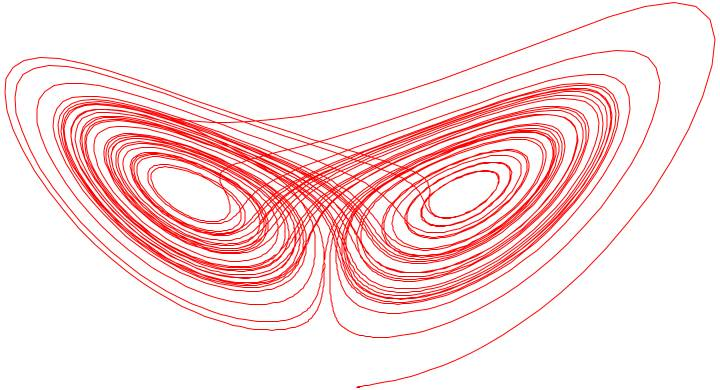
\includegraphics[scale=0.25]{lorenz.jpg}\\
		\caption{This is a blurry figure}
		\label{fig:a-nice-figure}
	\end{figure}

	\hyperlink{frame:previous-page}{\beamerbutton{Previous page}}  \hfill 	\hyperlink{frame:final-page}{\beamerbutton{Final page}} 
	
\end{frame}

\begin{frame}{And this is the final page}{Hooray!}\label{frame:final-page}
	
	Do not hesitate go give me feedback, raise issues, or even pull request on \href{}{Github}
	
\end{frame}

\section{Enjoy!}
\end{document}